\chapter{Bausteinsicht}
In diesem Kapitel zeigen wir den Aufbau des Condition Monitoring Systems. Es werden dabei die grundlegenden Pakete, Programmstrukturen und Komponenten beschrieben.
\section{Ebene 1}
Die Bausteine der ersten ebene sind zu implementierende Einheiten. Dazu gehört das Daten IO-Module, das Controller-Module und das Applikation-Präsenter-Modul. 
Die verschiedenen Module enthalten unterschiedliche Architekturstile, wordurch unser Gesamtsystem eine heterogene Softwarearchitektur aufweist. Jedes Modul verantwortet einen Teil der Gesamtfunktionalität. Anhand dieser werden die folgenden Ebenen um weitere Einheiten erweitert. Die folgende Grafik gibt einen ersten Überblick über das System.
\begin{figure}[h]
	\centering
	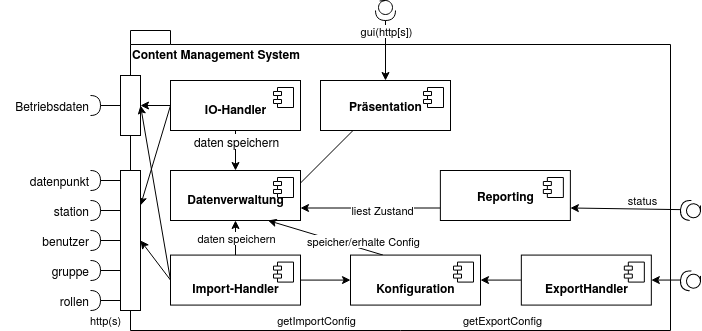
\includegraphics[width=1.0\textwidth]{Graphics/bausteinansicht_ebene_1.png}
	\caption{Bausteinsicht Level 1}
	\label{fig:bausteinsichtlvl1}
\end{figure}

Das Architekturziel hohe Performance zu gewährleisten wird von der Komponente IO-Modul verantwortet.
Das Controller-Modul, stellt sicher, dass das Architekturziel der Verfügbarkeit eingehalten wird. 
Das Applikation-Präsenter-Modul verantwortet, dass das Architekturziel der Benutzerfreundlichkeit eingehalten wird.
Die folgenden Abschnitte beschreiben die in der Abbildung dargestellten Einheiten von links nach rechts.  
\subsection{IO-Module}
\begin{table}
	\begin{tabularx}{\textwidth}{p{5cm} X}
		\hline
		 Zweck/Verantwortlichkeit & Das Modul nimmt über Außenschnittstellen Daten von Fremdsystemen entgegen und ist für deren korrekte persistente Speicherung verantwortlich  \\
		 \hline
		 Schnittstellen intern & Speichert Konfigurationsdaten und Rohdaten in Datenbank \\
		 \hline
		 Schnittstellen extern & Eingang von Rohdaten(csv, json, binär) und Konfigurationsdaten(Datenpunkt, Station, Benutzer, Gruppe, Rollen, Regeln) \\
		 \hline
	\end{tabularx} 
	\caption{IO-Module}
	\label{tab:IO-Module}
\end{table}

\subsection{Controller-Module}
\begin{table}[th]
	\begin{tabularx}{\textwidth}{p{5cm} X}
		\hline
		Zweck/Verantwortlichkeit & Verwaltet sämtliche Daten und beinhaltet Funktionsblöcke die Verwaltungsoperationen Lesen, Schreiben und Löschen bereitstellen. \\
		\hline
		Schnittstellen intern & Liefert und erhält Daten von dem Daten-IO-Module und stellt diese dem ApplikationPresenter-Module bereit\\
		\hline
	\end{tabularx} 
	\caption{Controller-Module}
	\label{Controller-Module}
\end{table}

\subsection{Applikation-Präsenter-Modul}
\begin{table}[th]
	\begin{tabularx}{\textwidth}{p{5cm} X}
		\hline
		Zweck/Verantwortlichkeit & Anzeigeoberflächenverwaltung für Benutzer \\
		\hline
		Schnittstellen & Nutzt den Webserver des Controller-Moduls\\
		\hline
	\end{tabularx} 
	\caption{Applikation-Präsenter-Modul}
	\label{tab:Applikation-Präsenter-Modul}
\end{table}
\clearpage
\section{Ebene 2}
\begin{figure}[h]
	\centering
	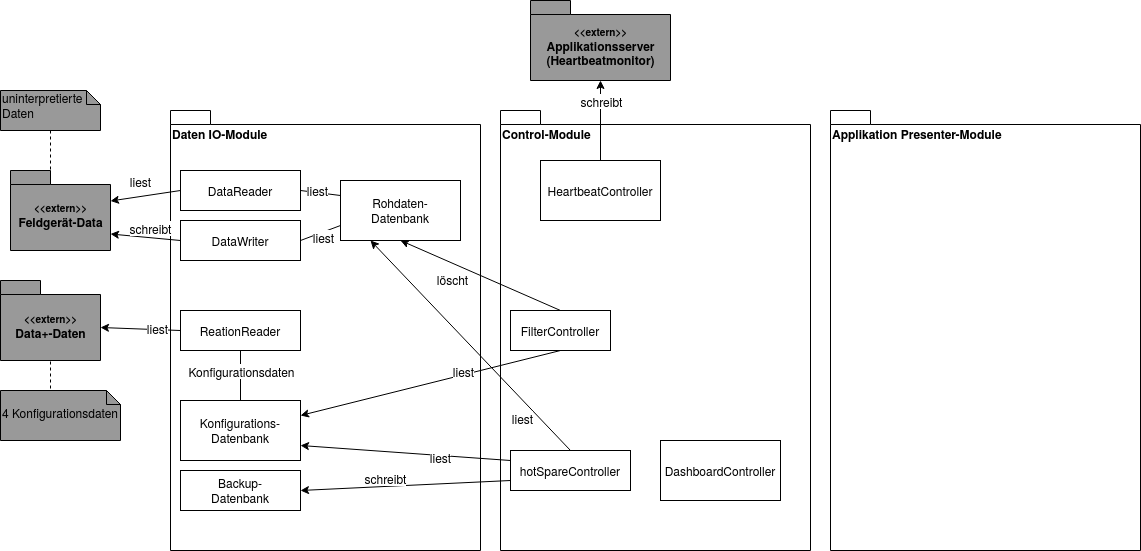
\includegraphics[width=1\textwidth]{Graphics/bausteinansicht_ebene_2.png}
	\caption{Bausteinsicht Level 2}
	\label{fig:bausteinsichtlvl2}
\end{figure}
Das Webinterface hat zu beiden Datenbanken eine Verbindung und kann auch die API des Filtermoduls mitbenutzen. In der Nutzeroberfläche wird zwischen einem administrativem und einem anwendungsspezifischen Teil unterschieden. In letzterem werden nur Daten und Statistiken aufbereitet angezeigt, während die Rechtevergabe und Feineinstellung in der Administratoroberfäche stattfindet. 

                 
                 
%Damit die die vielen Fremdsysteme und Maschinen mit unserer Software kommunizieren können, benötigen wir Implementierungen aller Protokolle in C++. Für CAN bzw. CANopen hat Alex eine Bibliothek in seiner Bachelorarbeit geschrieben. Für TCP/RTU nutzen wir Qt, für S7 gibt es Snap7. Die Hydac hat ihre eigene API und Bibliothek für die eigenen HFI-MM und HFI-CM Protokolle. Zu guter Letzt serialisieren wir WebSocket und HTTP mit Capn Proto. Alle Bibliotheken ermöglichen das einfache Abspeichern in den Wide-Column-Store oder bereiten es zumindest vor. Dafür werden eine DatenpunktID und StationsID der Maschine mit dem Wert und dem Zeitstempel gespeichert. Da diese Daten komplett ungeprüft in die Datenbank einfließen, muss ein weiterer Baustein alle Einträge überprüfen und Messfehler oder kritische Werte direkt in der Weboberfläche anzeigen. Dass die Überprüfung eventuell etwas langsamer als der Datenstrom in die Datenbank sein kann, ist an sich nicht schlimm, da die Anwendung in Produktionspausen aufholen und die noch ungeprüften Daten währenddessen verarbeitet.In der relationalen Datenbank befinden sich dann die DatenpunktIDs mit ihren Typen und Formaten, damit man ein Schema zur Darstellung im Interface hat. zusätzlich zu den Nutzer- und Rechtedaten gibt es auch noch eine Tabelle, die Regeln für die Datenpunkte abbildet.\\